%------------------------------------------------------------------------- 
\Section{Detail Sections}
\label{sec:architecture}
Loops are not compiled the first time they are called. VMKit maintains a loop count,which is incremented every time the loop executed.  VM interprets a loop until its call count exceeds a predefined trace\_JIT threshold value. So, most frequent loops(hot) are compiled as soon as VM started, loops which are executing less than threshold value will not be compiled by JIT. The threshold value could be selected to obtain significant balance between start-up times and run-time performance.\\
After particular loop is compiled, its call count will be reset to zero. Subsequent calls to the loop continue to increment its count. When the call count reaches its trace\_JIT threshold again it will be compiled by applying more optimization methods. This scenario will be occurred on some methods during an aggressive call by VM. So, high frequent loops will be more optimized than the normal less frequent routine.

\begin{figure}[ht!]
\centering
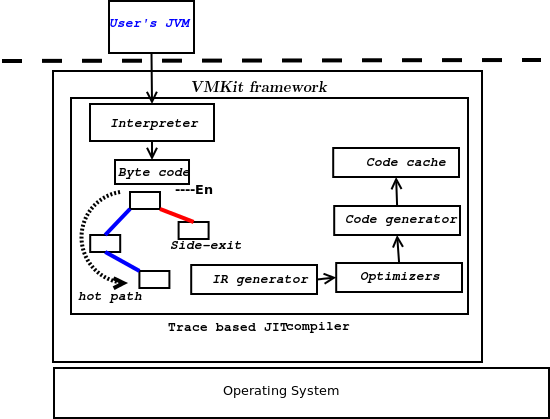
\includegraphics[width=70mm]{compiler.png}
\caption{Trace based JIT for VMKit}
\label{fig:architecture}
\end{figure}

Fig 1 explains how trace based JIT will lay down in VMKit. Even though VMKit composed with other components , diagram shows only JIT components which has derived from LLVM. As number of loop execution is counting by JIT when the counter reaches a threshold, the interpreter will be starting trace process. According to above diagram tracing process will be started at place -En and when tracing process reaches  back to the address where the tracing started, the interpreter stops tracing and the compiler compiles the trace to native code. The path in blue may or may not be an actual hot path since interpreter is not doing an perfect path profiling. Guard control will be applied when instructions are deviated from actual hot path. During the interpretation , if a Guard is triggered , the native code use side-exit and back to normal interpretation mechanism. There are some other advanced way to deal with frequent side-exit which would make side-exit path to separate branch of hot-path ~\cite{arch2}.

